\section{Case Study: Shopping Carts}
\label{sec:carts}

\begin{figure}[t]
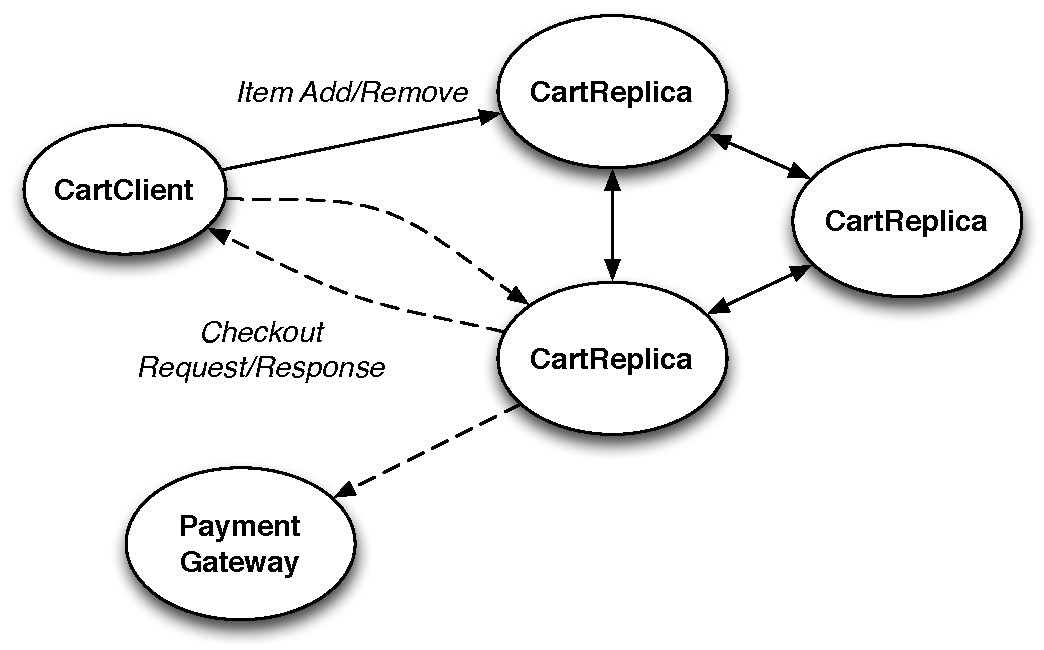
\includegraphics[width=\linewidth]{fig/cart_arch.pdf}
\caption{Architecture of a simple shopping cart system.}
\label{fig:cart-system-arch}
\end{figure}

The next two sections contain case studies that show how \lang can be used to
build practical distributed programs. Our goal is to demonstrate that
non-trivial distributed protocols can be expressed using lattices and monotone
functions. If written in Bloom, these programs would be considered non-monotonic
because they contain aggregation. Presenting monotonic implementations in \lang
is equivalent to showing that the use of aggregation in these protocols is
``safe'' and produces consistent results without needing additional
coordination.

In the first case study, we consider a simple e-commerce system in which clients
interact with a shopping cart service by adding and removing items over the
course of a shopping session (Figure~\ref{fig:cart-system-arch}). The cart service is
replicated to improve fault tolerance; client requests can be routed to any of
the cart replicas. Eventually, a client submits a ``checkout'' operation, at
which point the cumulative effect of their shopping session should be summarized
and returned to the client. In a practical system, the result of the checkout
operation might be presented to the client for confirmation or submitted to a
payment processor to complete the e-commerce transaction. This case study is
based on the cart system from Alvaro et al.~\cite{Alvaro2011}, which was in turn
inspired by the discussion of replicated shopping carts in the Dynamo
paper~\cite{DeCandia2007}.

Alvaro et al.\ discuss two different designs: a ``disorderly'' version in which
the cart state is represented as a set of operations (allowing monotonic
accumulation of adds and removes) and a ``destructive'' version in which the
cart state is managed by a key-value store, which requires a non-monotonic
update on each cart action.

\subsection{Monotonic checkout}
\label{sec:monotone-checkout}

\begin{figure}[t]
\begin{scriptsize}

\begin{lstlisting}
module CartProtocol
  state do
    channel :action_msg,
      [:@server, :session, :reqid] => [:item, :cnt]
    channel :checkout_msg,
      [:@server, :session, :reqid] => [:lbound, :addr]
    channel :response_msg,
      [:@client, :session] => [:summary]
  end
end

module MonotoneReplica
  include CartProtocol

  state { lmap :sessions }

  bloom do
    sessions <= action_msg do |m|
      c = LCart.new({m.reqid => [ACTION, m.item, m.cnt]}) (*\label{line:cart-action-op}*)
      { m.session => c }
    }
    sessions <= checkout_msg do |m|
      c = LCart.new({m.reqid => [CHECKOUT, m.lbound, m.addr]}) (*\label{line:cart-checkout-op}*)
      { m.session => c }
    }

    response_msg <~ sessions do |session, c| (*\label{line:cart-response-start}*)
      c.is_complete.when_true {
        [c.checkout_addr, session, c.summary]
      }
    end (*\label{line:cart-response-end}*)
  end
end
\end{lstlisting}
\end{scriptsize}
\caption{\lang program for a server replica that allows checkout to be a
  monotone (coordination-free) operation.}
\label{fig:monotone-cart}
\end{figure}

For both the ``disorderly'' and ``destructive'' designs, Alvaro et al.\ argue
that processing a checkout request is non-monotonic because it requires
aggregating over an asynchronously computed data set---in general, coordination
might be required to ensure that all inputs have been received before the
checkout response can be returned to the client. However, observe that the
client knows exactly which add/remove operations should be reflected in the
result of the checkout. If that information can be propagated to the cart
service, any server replica can decide if it has enough information to process
the checkout operation without needing additional coordination. This design is
monotonic: once a checkout response is produced, it will never change or be
retracted. Our goal is to translate this design into a monotonic \lang program.

% This can be done by assigning IDs to each message sent by the client. Each
% client has a session ID; within a session, operation IDs are assigned in
% increasing numeric order without gaps. Hence, if the client sends a ``lower
% bound'' message ID along with the checkout message, any replica of the cart
% service can independently ensure that it only produces a response message once
% it has received all the operations in the ID range indicated by the client. This
% essentially requires a threshold test over the operation IDs received by a given
% replica, which can easily be implemented using \lang.

Figure~\ref{fig:monotone-cart} contains the server code for this design (we omit
the client code for the sake of brevity). Communication with the client occurs
via the channels declared in the \texttt{CartProtocol} module. We represent the
state of a server replica using an \texttt{lmap} lattice that associates session
IDs with \texttt{lcart} lattice elements. \texttt{lcart} is a custom lattice
that represents the state of a single shopping cart. An \texttt{lcart} contains
a set of client operations. Each operation has a unique ID; operation IDs are
assigned by the client in increasing numeric order without gaps. An
\texttt{lcart} contains two kinds of operations, \emph{actions} and
\emph{checkouts}. An action describes the addition or removal of an item from
the cart. An \texttt{lcart} contains at most one checkout operation---the
checkout specifies the smallest operation ID that must be reflected in the
result of the checkout, along with the address where the checkout response
should be sent.  Lines~\ref{line:cart-action-op} and \ref{line:cart-checkout-op}
construct \texttt{lcart} elements that contain a single action or checkout
operation, respectively. These singleton carts are then merged with the previous
cart state associated with the client's session, if any.

An \texttt{lcart} is \emph{complete} if it contains a checkout operation as well
as all the actions in the ID range identified by the checkout. Hence, testing
whether an \texttt{lcart} is complete is a monotone function: it is similar to
testing whether an accumulating set has crossed a threshold. Hence, if any
server replica determines that it has a complete cart, it can send a response to
the client without risking inconsistency. Without coordination, the client might
receive multiple responses but they will all reflect the same cart contents.

Note that the statement that produces a response to the client
(lines~\ref{line:cart-response-start}--\ref{line:cart-response-end}) is
contingent on having a complete cart. \texttt{summary} is a monotone method that
returns a summary of the actions in the cart---an exception is raised if
\texttt{summary} is called before the cart is complete. Similarly, attempts to
construct ``illegal'' \texttt{lcart} elements (e.g., carts containing multiple
checkout operations or actions that are outside the ID range specified by the
checkout) also result in runtime exceptions, since this indicates a likely logic
error in the program. Implementing the \texttt{lcart} lattice required 58 lines
of Ruby using the lattice API described in Section~\ref{sec:lattice-api}.

% Note that because each replica determines when the cart is ``complete''
% independently, multiple response messages may be produced. However, they will
% all be consistent, because ...

% \subsection{Performance Study}
% \begin{itemize}
% \item
%   goal: demonstrate that removing coordination from a distributed protocol can
%   significantly reduce its running time
% \item
%   benchmark: destructive cart w/ coordination on each action vs.\ destructive
%   cart in \lang without coordination, disorderly cart with coordination on
%   checkout vs.\ disorderly cart with monotonic checkout
% \end{itemize}
